\chapter{Rotor-fuselage dynamic coupling}
\label{ch:Rotor-fuselage dynamic coupling}

\subsection*{Rotating systems}
\addcontentsline{toc}{subsection}{Rotating systems}
\noindent
\underline{The rotation of the tail-rotor}, which is obviously spinning during the flight condition, \underline{considerably affect the vibrational behaviour of the tailboom} with respect to the case in which the rotor is still (for example on the ground with engine off). \\
In rotating systems, in fact, the dynamic behaviour undergoes considerable variations due to the fenomena related to the rotation of the systems, which are basically:
\begin{itemize}
	\item the onset of \textbf{gyroscopic moments}, function of the angular velocity $\Omega$;
	\item the presence of \textbf{static} or \textbf{dynamic} unbalances which produces excitations also function of $\Omega$. 
\end{itemize}

\noindent
The consequence of those phenomena is that the whole system, at each angular velocity, has natural frequencies different from those relative to the system in rest and those frequencies results also variable with $\Omega$. \\
\noindent
Furthermore, when the rotor system is fixed on the tailboom, the two systems dynamically interact to each other and those effects must be taken into account in order to accurately model the real system's dynamic behaviour. \\

\noindent
In the literature, there have been many attempts to predict the vibration of a rotor-body coupled system with a variety of assumptions and solution methods; anyway, from most of those past studies \underline{there appears to be no viable alternative to carrying out a coupled} \underline{rotor-fuselage analysis when one is investigating fuselage response to rotor excitation}, in order to represent accurately the real system's behaviour. \\

\noindent
So, 3 possible ways to treat the coupling will be presented in the next section which is only intended as possible hints to extend this project for further improvements.  


\clearpage
\section*{Hints on possible approaches}
\addcontentsline{toc}{subsection}{Hints on possible approaches}
\noindent
The fuselage's equations of motion and the rotor's ones results to be coupled. \\
There are different possible approaches to solve a coupled problem:

\medskip
\subsubsection*{a) Complete Coupled Formulation}
\addcontentsline{toc}{subsubsection}{a) Complete Coupled Formulation}
\noindent
In this case, all the linear terms of the rotor and fuselage equations are transferred from the right hand side to the left hand side of the equation.

\smallskip
\begin{figure}[h]
	\begin{center}
		\centering  		 		
		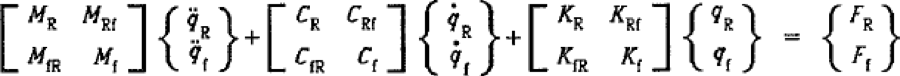
\includegraphics[width=0.9\linewidth]{PICTURES/3b_coupling/eq_1.png}
	\end{center}
	\caption {Complete coupled formulation equations}
\end{figure}
%\vspace{0.5cm}


\underline{Advantage}: 
\begin{itemize}
	\item Direct evaluation of the eigenvalues and eigenvectors of the system;
\end{itemize}



\underline{Disadvantages}: 
\begin{itemize}
	\item Inflexibility of changing any of the terms;
	\item It require linearization of the force terms which lead to additional assumptions and approximations.
\end{itemize}

\medskip
\subsubsection*{b) Explicit Coupled Formulation}
\addcontentsline{toc}{subsubsection}{b) Explicit Coupled Formulation}
\noindent
This second approach is based on an advanced technique for solving non-linear sets of equations. The rotor/body coupled system of equations are formulated in the following explicit form:

\smallskip
\begin{figure}[h]
	\begin{center}
		\centering  		 		
		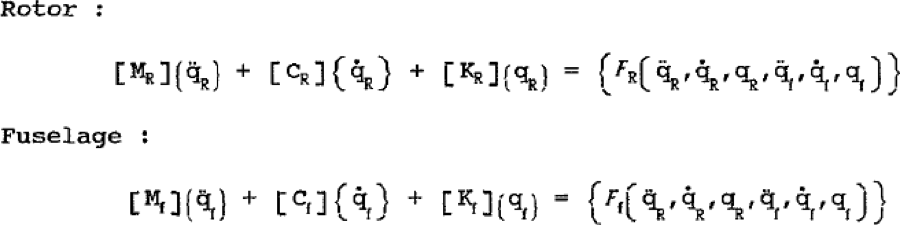
\includegraphics[width=0.9\linewidth]{PICTURES/3b_coupling/eq_2.png}
	\end{center}
	\caption {Explicit coupled formulation equations}
\end{figure}
%\vspace{0.5cm}

\noindent
Here the rotor/fuselage coupling terms lie on the right hand side with external forces. Therefore the right hand terms are function of the rotor as well as fuselage motion. Rotor and fuselage equations are solved iteratively. The converged solution represents a fully coupled system.

\medskip
\underline{Advantages}: 
\begin{itemize}
	\item Flexibility in changing the fuselage modelling;
	\item It is possible to identify the coupling terms in the forcing expression.
\end{itemize}

\underline{Disadvantage}: 
\begin{itemize}
	\item direct evaluation of the coupled system eigenvalues and eigenvectors has to be done only by frequency sweep;
	\item requires a non-linear solver
\end{itemize}


\bigskip
\subsubsection*{c) Simulate gyroscopic effects with rotational springs}
\addcontentsline{toc}{subsubsection}{c) Simulate gyroscopic effects with rotational springs}
\noindent
This third case, consists in simplifying the problem considering the rotor as a concentrated mass and inertia and introducing \underline{rotational springs} that act on the fuselage for modeling the gyroscopic effects that appears when moments or forces act on the spinning rotor making it rotate around on of its axes. 

\medskip
\underline{Disadvantages}: 
\begin{itemize}
	\item It is an approximation; even introducing an equivalent rotor mass, although it gives a somewhat
	better approximation, still does not adequately represent the coupled rotor-fuselage system;
	\item Rotational springs musts apply a moment in a plane orthogonal to the one in which the rotation occours (difficult to implement);
	\item Stiffness properties of the springs are not constant  (vary with the rotor's speed $\Omega$).
\end{itemize}


\bigskip
\noindent
The first two methods have been taken from literature from a NASA research article (cited in the bibliography) while the third method is just a proposal in order to simplify and treat this complex problem in a easier way. \\
Many other methods can be found in literature to solve this particular problem and each of them has different assumptions and limitations. The choice in one of them depends on project's purposes and expectations.


\clearpage
\subsection*{Effect of the rotor-fuselage dynamic coupling on the system's natural frequencies}
\addcontentsline{toc}{subsection}{Effect of the rotor-fuselage coupling}
\noindent
In the following pictures, taken from the literature, it is outlined the effect of the rotor-fuselage dynamic coupling on the system's resonant frequencies. \\
It is is clear that the dynamic coupling cannot be neglected if an accurate model is needed. In fact, it is evident that system's natural frequencies significantly change with rotor's speed and at each speed they are different from the frequencies at still condition. \\

\smallskip
\begin{figure}[h]
	\begin{center}
		\centering  		 		
		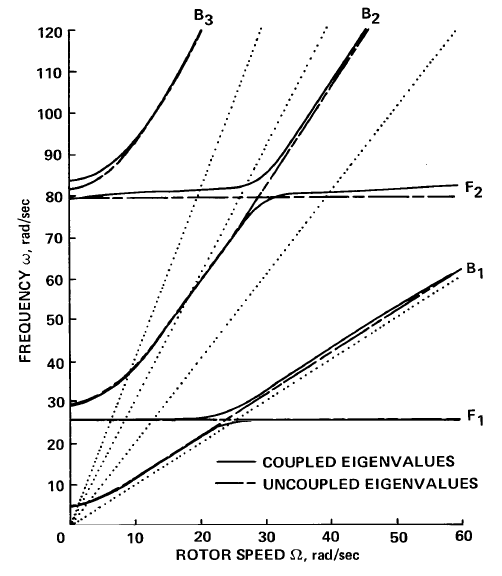
\includegraphics[width=0.85\linewidth]{PICTURES/3b_coupling/1.png}
	\end{center}
	\caption {Coupled and uncoupled rotor-fuselage eigenvalues}
\end{figure}
